\section{Interceptor}
\label{sec:interceptor}

The interceptor architectural pattern allows services to be added transparently to a framework and triggered automatically when certain events occur.


\subsection{Begriffe}

\begin{itemize}
	\item \emph{Application}: Implementiert Framework
	\item \emph{Interceptor}: Klasse/Objekt welche eine Schnittstelle zum Intercepten definiert
	\item \emph{Concrete Interceptor}: Klasse/Objekt welche den Interceptor implementiert
	\item \emph{Concrete Framework}: Instanziertes Framework (konkrete Implementation eines Frameworks)
	\item \emph{Black-Box-Framework}: Framework deren Source nicht zugänglich ist / nicht modifizierbar ist
\end{itemize}


\subsection{Kontext}

Frameworks welche transparent erweitert werden können.


\subsection{Problem}

Frameworks können nicht voraussehen, welche Services ihre User benutzen müssen/wollen und User können insbesondere Black-Box Frameworks nicht erweitern, wenn sie nicht ursprünglich dafür gedacht waren.
Frameworks müssen daher Integrationen von Dritt-Services ohne Modifikation der Architektur erlauben. Auch sollen solche Modifikationen keine existierenden Framework-Komponenten oder Applikationen des Frameworks beeinflussen.


\subsection{Lösung}

Applikationen welche bestimmte Frameworks einsetzen müssen sich daher transparent beim Framework für bestimmte Services oder Events registrieren können. Durch die Implementation von bestimmten Schnittstellen, welche das Framework zur Verfügung stellt, muss die Applikation einzelne Aspekte des Frameworks kontrollieren und auf das Framework zugreifen können.


\subsection{Implementation}

Das Interceptor Callback Interface ist dabei eine Implementation zu diesem Problem. Das Framework stellt dieses Interface zur Verfügung und Applikationen können concrete interceptors aufgrund dieses Interfaces implementieren. Diese Klassen registrieren sie bei einem Dispatcher für bestimmte Ereignisse und werden danach vom Framework mit context Objekten aufgerufen.
Typischerweise existiert ein Dispatcher pro Interceptor.

\begin{figure}[H]
	\centering
	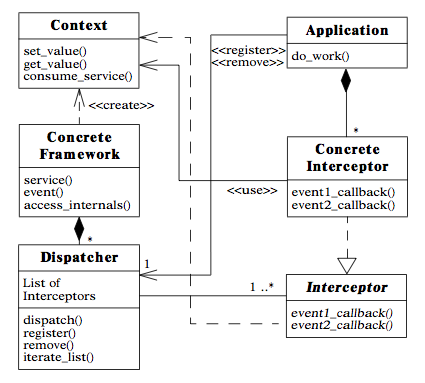
\includegraphics[width=12cm]{content/posa2/interceptor/images/uml-diagram.png}
	\caption{Interceptor UML-Diagramm}
\end{figure}


\subsection{Varianten}
\begin{itemize}
	\item \emph{Interceptor}\\
	Wird häufig auf der Server-Seite von Verteilten Systemen verwendet. Dabei wird ein Proxy (POSA1) instanziert, welcher eine Referenz auf das concrete framework bzw. den lokalen server hält. Sobald ein Client eine Anfrage macht, erhält das Proxy-Objekt diesen und führt u.U. Pre-Processing Funktionalität aus. Danach wird es dem Lokalen Server übergeben, welcher dann wiederum mittels dem Proxy dem Client antwortet.
	\item \emph{Single Interceptor-per-Dispatcher}\\
	Diese Variante erlaubt nur die Registration einem Interceptor pro Disptacher. Diese Restriktion kann die implementation vereinfachen.
	\item \emph{Interceptor Factory}\\
	Wenn das Framework die gleiche Klasse mehrere Male instanziert. Statt dass für jedes Objekt die Registration auf dem Dispatcher geschieht, werden Factories registriert, welche dann vom Framework aufgerufen werden.
	\item \emph{Implicit Interceptor Registration}\\
	Statt explizit Interceptors beim Dispatcher zu registrieren, kann das Framework auch Methoden zur Verfügung stellen, um dynamisch an spezifischen Orten oder mittels Konfigurationen (Component Configurator) diese automatisch zu registrieren.
\end{itemize}


\subsection{Verwendung}

\begin{itemize}
	\item \emph{Component-based application servers}
	\item \emph{CORBA} implementation
	\item \emph{COM}
	\item \emph{Web Browsers} (Extensions)
	\item \emph{Reference Monitor} (Security Patterns)
\end{itemize}


\subsection{Vorteile}

\begin{itemize}
	\item Extensibility/Flexibility des Frameworks
	\item Separation of Concerns
	\item Monitoring und Kontrolle eines Frameworks unterstützen
	\item Layer symmetry: Durch Interceptors pro Layer können verschiedene Zusatzfunktionalitäten transparent implementiert werden
	\item Reusability
\end{itemize}


\subsection{Nachteile}

\begin{itemize}
	\item Architektur/Design wird komplexer
	\item Fehlerbehaftete Interceptors können die gesamte Applikation blockieren
	\item Interception cascades: Wenn ein Interceptor eine Änderung in einem Kontext-Objekt bewirkt kann das weitere Events zur Folge haben, welche weitere Interceptors triggern können
\end{itemize}
